\documentclass[12pt,a4paper,twoside]{article}
\usepackage[T1]{fontenc}
\usepackage[utf8]{inputenc}
\usepackage[polish]{babel}
\usepackage{graphicx}
\usepackage{amsmath}
\usepackage{times}
\usepackage{indentfirst}
\usepackage[left=3cm,right=2cm,top=2.5cm,bottom=2.5cm]{geometry}
\usepackage{natbib}
\usepackage{enumitem}
\usepackage{color}
\usepackage{tikz}
\usepackage{booktabs}
\usepackage{tabulary}
\usepackage{url}
\urlstyle{same}
\setlist{itemsep=0pt}
\setlist{nolistsep}
\frenchspacing
\linespread{1.5}
\addto\captionspolish{%
\renewcommand*\listtablename{Spis tabel}
\renewcommand*\tablename{Tabela}
}
\usepackage{titlesec}
\titlelabel{\thetitle.\quad}
\usepackage{etoolbox}
\makeatletter
\patchcmd{\ttlh@hang}{\parindent\z@}{\parindent\z@\leavevmode}{}{}
\patchcmd{\ttlh@hang}{\noindent}{}{}{}
\makeatother
\setlist[itemize]{leftmargin=*}

\begin{document}

\begin{center}

  
\includegraphics[scale=0.3]{../obrazy/sgh_full.png}

  \vspace{1cm}
  Studium magisterskie

\end{center}

\vspace{1cm}

\noindent Kierunek: Analiza danych - big data

\noindent Specjalność: \dots

\vspace{1cm}

{
\leftskip=10cm\noindent
Roni Chikhmous\newline
Nr albumu: 69684

}

\vspace{2cm}

\begin{center}
  \LARGE
  Optymalizacja kosztowa procesu konstruowania głębokich sieci neuronowych (ang. deep neural networks) z wykorzystaniem chmury obliczeniowej
\end{center}

\vspace{1cm}

{
\leftskip=10cm\noindent
Praca magisterska napisana\newline
w Instytucie Ekonometrii\newline
pod kierunkiem naukowym\newline
dr. Przemysława Szufla

}

\vfill

\begin{center}
Warszawa, 2017
\end{center}
\thispagestyle{empty}

\clearpage
\thispagestyle{empty}
\mbox{}

% druga strona będzie pusta, ponieważ drukujemy dwustronnie
\clearpage

\tableofcontents

\clearpage

\section{Wprowadzenie}
\noindent
Celem niniejszej pracy jest zaproponowanie metody wyznaczania optymalnego kosztowo sposobu generacji struktur głębokich sieci neuronowych (ang. \textit{deep neural networks}). Uczenie tego typu modeli wymaga znacznej mocy obliczeniowej, dostępnej na żądanie i na krótki czas. To sprawia, że tradycyjne rozwiązania (takie jak architektura \textit{on premises}) nie są optymalne kosztowo, por. \citet{armburst2010}, \citet{oecd2014}. Rozwiązaniem, które odpowiada na wymienione potrzeby jest model \textit{pay-as-you-go} wykorzystywany w usługach przetwarzania w chmurze (ang. \textit{cloud computing}).

Odkrycia naukowe ostatnich lat w dziedzinach uczenia maszynowego i sztucznej inteligencji wpłynęły pozytywnie na ich popularność i liczbę potencjalnych zastosowań \citep{lecun2015}. Szczególna uwaga poświęcana jest sieciom neuronowym, które, choć pozwalają na rozwiązywanie dotychczas problematycznych zagadnień \citep{lecun2015}, są algorytmami wymagającymi znacznej ilości danych i mocy obliczeniowej, por. \citet{krizhevsky2012} i \citet{srivastava2014}. Ośrodki naukowe we współpracy z największymi firmami technologicznymi, jak Google czy Microsoft wykorzystują owe modele \citep{goodfellow2016} do rozwiązywania szeregu problemów takich jak klasyfikacja obrazów (\citet{krizhevsky2012}; \citet{shetty2016}; \citet{szegedy2014}; \citet{chen2016}) i przetwarzanie języka naturalnego \citep{hinton2012}. Kluczowa zaleta głębokich sieci neuronowych polega na możliwości budowania modelu z wykorzystaniem nieprzetworzonych danych. W przypadku klasycznych algorytmów \textit{machine learningowych}, konieczna jest inżynieria cech i ręczna ich ekstrakcja, podczas gdy wielowarstwowe sieci neuronowe są metodą, która w sposób automatyczny wykrywa występujące w zbiorach danych schematy, zależności, por. \citet{girschick2014}, \citet{gysel2016} i \citet{mnih2013}. Przykładowo, w przypadku klasyfikacji obrazów, pierwsza warstwa sieci neuronowej odpowiada za detekcję ogólnych jego cech, takich jak umiejscowienie krawędzi w kluczowych miejscach. Kolejna odpowiada za analizowanie ich położenia wzgledem siebie i wykrywanie pewnych motywów. Co do zasady, pierwsze warstwy odpowiadają za ogólne cechy przetwarzanych danych, podczas gdy każda kolejna ma za zadanie przechodzić na wyższy poziom szczegółowości.


Na popularności zyskało wykorzystywanie procesorów graficznych (ang. \textit{Graphics Processing Unit, GPU}) oferowanych przez Nvidia do poprawy wydajności procesu generacji tego typu struktur (\citet{jermain2015}; \citet{litvinenko2014}; \citet{strom2015}; \citet{vanhoucke2011}). Ponadto, giganci technologiczni inwestują w poszukiwanie potencjalnych sposobów na dalsze usprawnienie tego procesu, takich jak wykorzystanie bezpośrednio programowalnych macierzy bramek (ang. \textit{Field-Programmable Gate Array}) czy rozwiązania opracowanego przez Wave Computing - \textit{Dataflow Processing Unit (DPU)}, por. \citet{gysel2016}; \citet{chen2016}; \citet{han2016}.

Zarówno przeprowadzanie symulacji w chmurze, wykorzystywanie procesorów graficznych w celu poprawy wydajności generacji głębokich sieci neuronowych, jak i porównania poszczególnych jednostek były przedmiotem badań, por. \citet{calheiros2010}, \citet{github2017}, \citet{medium2017b}, \citet{hackernoon2017}. Nie przeprowadzono jednak analizy oszczędności czasowych wynikających ze stosowania \textit{GPU} w chmurze i brak jest odpowiedzi na pytanie, czy rekompensują one ich wyższą cenę w porównaniu do klasycznych jednostek.

Zatem, w pracy badane będą następujące hipotezy:
\begin{itemize}
\item stosowanie jednostek wykorzystujących GPU jest rozwiązaniem efektywnym kosztowo  w porównaniu do jednostek wyposażonych wyłącznie w CPU,
\item wynajem jednostek AWS P2 jest efektywniejsze kosztowo od jednostek oferowanych przez Microsoft Azure oraz Google Cloud,
\item wykorzystywanie opracowanego narzędzia do wyboru rodzaju jednostki obliczeniowej pozwala na optymalizację kosztową procesu generacji głębokich sieci neuronowych.
\end{itemize}

Pierwsza hipoteza porusza kwestię efektywności kosztowej jednostek GPU oferowanych w chmurze. Literatura dostarcza dowodów, że stosowanie tego typu jednostek prowadzi do
krótszego czasu konstruowania sieci neuronowych, por. \citet{jermain2015} i \citet{litvinenko2014}. Nie jest jednak oczywistym, czy efektywniejszym kosztowo rozwiązaniem w przypadku architektury chmurowej są jednostki GPU czy CPU. Pomimo niższego czasu potrzebnego na estymację modelu, cena jednostek wyposażonych w GPU może być
na tyle wysoka, że ich wynajem nie jest optymalny w sensie kosztowym.

Następnie chcemy skupić się na porównaniu ofert różnych dostawców usług przetwarzania w chmurze. Dokonamy porównania efektywności kosztowej jednostek wyposażonych w procesory graficzne, dostarczanych przez Amazon, Microsoft oraz Google.

Efektem pracy będzie dostarczenie narzędzia przeprowadzającego eksperymenty i pozwalającego na wybór najefektywniejszej kosztowo jednostki obliczeniowej. To narzędzie ma na
celu przeprowadzenie optymalizacji kosztowej w zależności od rozważanych jednostek obliczeniowych i przedstawionego problemu.

Na podstawie prezentowanego badania zostanie wybrany zbiór decyzji niezdominowanych (optymalnych w sensie Pareto) dla rozważanego problemu wielokryterialnego. Eksperyment przeprowadzany będzie poprzez dokonywanie wielokrotnych, empirycznych pomiarów dla każdej rozważanej jednostki obliczeniowej. Wynikiem każdego pomiaru będzie koszt wynajmu serwera oraz czas potrzebny na skonstruowanie modelu. Wybranym do przeprowadzania eksperymentu problemem jest przetwarzanie obrazu (stworzenie klasyfikatora). Następnie przeprowadzimy agregację otrzymanych wyników oraz analizy zbioru dostępnych decyzji, by ostatecznie przedstawić zbiór decyzji optymalnych w sensie Pareto.

\clearpage


\section{Deep learning w chmurze}
\subsection{Sieci neuronowe i deep learning}

Do najpopularniejszych przykładów użycia metod \textit{machine learningowych} zaliczyć można dostosowywanie wyników wyszukiwań internetowych, filtrowanie i personalizacja powiadomień w mediach społecznościowych, rekomendacje produktów i reklama internetowa, ale również rozpoznawanie dźwięku, identyfikowanie obiektów na obrazach i tłumaczenie tekstu. W tym rozdziale opisane zostaną algorytmy stosowane do ostatnich z wymienionych przypadków - głębokie sieci neuronowe (ang. \textit{deep neural networks}).

\subsubsection{Historia sieci neuronowych}

Wraz z nadejściem elektroniki i komputerów, badacze rozpoczęli podejmować próby replikacji ludzkich procesów myślowych na systemy logiczne. Choć pierwsze kroki w tej dziedzinie zostały podjęte przez \citet{mcculloch1943} oraz \citet{hebb1949}, istotny z punktu widzenia uczenia maszynowego przełom w sztucznych sieciach neuronowych został dokonany w pracy \citet{rosenblatt1957}, gdzie po raz pierwszy wprowadzono koncept perceptronu - algorytmu, który miał pozwolić na poprawne rozpoznawanie obrazów. Perceptron jest jednym z najbardziej podstawowych przykładów sieci neuronowych, jego schemat został przedstawiony na rysunku \ref{fig:perceptron}.

\begin{figure}[h]
  \centering
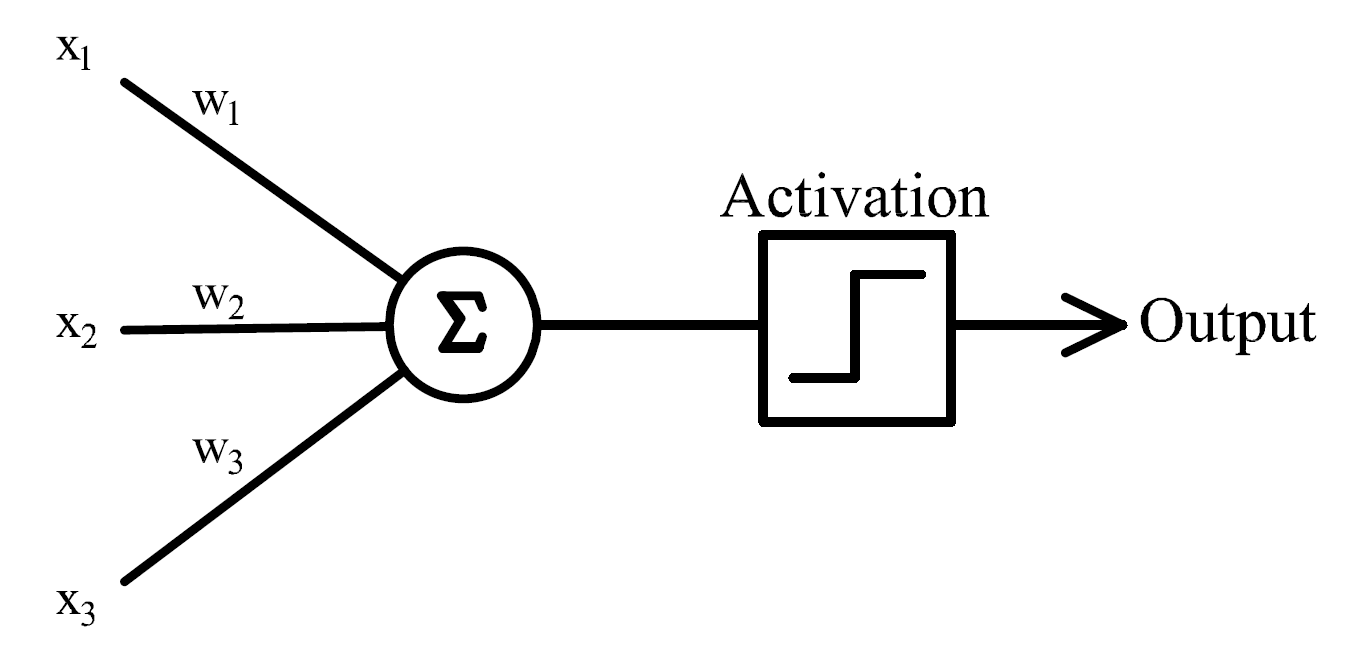
\includegraphics[scale=0.8]{../obrazy/fig:perceptron.png}
\caption{Pereceptron przedstawiony na przykładzie składa się z dwóch warstw – warstwy wejściowej z trzema wartościami wejściowymi (\(x_1, x_2, x_3 \)) oraz warstwy wyjściowej. \label{fig:perceptron}}
\end{figure}

Przyjmuje on wektor \(\mathbf{x}\) binarnych wartości wejściowych \(x_1, \ldots, x_n \). Każda z tych wartości wejściowych jest przyjmowana z wagą \(w_1, \ldots, w_n \), będącą liczbą rzeczywistą. Owe parametry można w intuicyjny sposób przedstawić jako wpływ (mający wartość i kierunek) każdego z sygnałów wejściowych na sygnał wyjściowy. Ostatecznie ważona suma wartości wejściowych porównywana jest z wartoscią progową (ang. \textit{threshold}), będącą kolejnym parametrem perceptronu. W przypadku, gdy ważona suma jest większa od wartości progowej, funkcja aktywacji zwraca wartość wyjściową 1, w przeciwnym wypadku zwraca 0. Przyjmując formalną reprezentację:
\begin{align}
  output=\begin{cases}
    0& \text{jeśli $\sum_j$ $w_j$ $x_j$ $<$ threshold},\\
    1& \text{jeśli $\sum_j$ $w_j$ $x_j$ $\geq$ threshold}.
  \end{cases}
\end{align}

\citet{widrow1960} przedstawili ADALINE - jednowarstwową sztuczną sieć neuronową, która uczona była za pomocą szczególnego przypadku wciąż wykorzystywanej metody optymalizacji opartej na gradiencie - \textit{stochastic gradient descent}.

Pomimo obiecujących początków i optymizmu towarzyszącemu nowemu odkryciu, badania nad sztucznymi sieciami neuronowymi zostały w dużej części porzucone za sprawą publikacji \citet{minsky1969}. Nakreślili oni granice możliwości modeli liniowych (w tym perceptronu i jednowarstwowych sieci neuronowych) jako systemu uczącego się. W szczególności udowodnili, że z wykorzystaniem tego typu algorytmów nie da się odwzorować funkcji logicznej XOR. Ich odkrycie zakończyło pierwszy okres popularności sieci neuronowych, zwany \textit{cybernetyką}.

Kolejna fala popularności została zapoczątkowana przez interdyscyplinarny ruch - koneksjonizm (ang. \textit{connectionism}), określany również jako modele PDP (równoległego rozproszonego przetwarzania informacji). Wiele idei wywodzących się z cybernetyki zostało w tym okresie zaadaptowanych do badań nad charakterem poznania, por. \citet{touretzky1985}. Jedną z nich jest pomysł rozproszonej reprezentacji \citep{hinton1986}. Przedstawia on założenie, że każdy sygnał wejściowy powinien być reprezentowany przez wiele cech systemu, a każda cecha powinna być włączona w tworzenie reprezentacji możliwie wielu sygnałów wejściowych. Koncept rozproszonej reprezentacji pozostaje kluczowym komponentem konstruowanych obecnie sieci neuronowych, por. \citet{goodfellow2016}. Oprócz przełomu na polu nauk poznawczych, do metod optymalizacyjnych również zostały wprowadzone nowe idee. Praca \citet{rumelhart1986} dowiodła empirycznie skuteczność wciąż stosowanego algorytmu propagacji wstecznej
(ang. \textit{backpropagation}) w przyspieszaniu procesu uczenia sieci neuronowych, co pozwoliło na wykorzystywanie ich do szerszego zakresu problemów. Jednakże, ruch koneksjonizmu utrzymywał zainteresowanie środowisk naukowych i biznesowych tylko do połowy lat 90. Nieproporcjonalne oczekiwania co do możliwości sztucznych sieci neuronowych oraz pojawienie się innych metod sprawiły, że inwestorzy wycofali swoje wsparcie.

Aktualne zainteresowanie sieciami neuronowymi zostało zapoczątkowane jako skutek badań nad modelami o skomplikowanej architekturze (\citet{hintonetal2006}; \citet{bengio2007a}). Wtedy też tego typu architektury sieci neuronowych otrzymały określenie \textit{głębokich}. Miało na celu podkreślenie faktu wykorzystywania wielu ukrytych warstw, co dotychczas nie było możliwe z powodu niedostatecznej mocy obliczeniowej. Istotność tej cechy w sieciach neuronowych jest podkreślana w pracach \citet{bengio2007b} i \citet{bengio2011}.





































































\clearpage

\subsection{Cloud computing}

\noindent
W tym rozdziale omówiony zostanie paradygmat przetwarzania danych w chmurze. Przedstawione zostaną jego kluczowe cechy, wymagania stawiane dostawcom i definicje często spotykanych pojęć. Następnie opiszemy najpopularniejsze modele świadczonych usług, modele implementacji i rozwiązania technologiczne leżące u podstaw opisywanego paradygmatu, by finalnie przejść do aspektów ekonomicznych i przybliżenia rynku \textit{cloud computingu} wraz z opisem największych dostawców.

\subsubsection{Definicje, kluczowe charakterystyki}

\noindent
Przetwarzanie danych w chmurze definiowane jest w pracach \citet{buyya2009} oraz \citet{calheiros2010} jako ,,rodzaj równoległego i rozproszonego systemu, składającego się z licznych, połączonych ze sobą i wirtualizowanych serwerów, która są dynamicznie przydzielane na podstawie ustaleń pomiędzy dostawcą a konsumentami, dokonanych za pośrednictwem dedykowanego serwisu''. Innymi słowy, w tym modelu pamięć, moc obliczeniowa znajdują się ,,w chmurze'', która jest zbiorem centrów danych (ang. \textit{data centers}), posiadanych oraz utrzymywanych przez zewnętrzny podmiot. Konsumenci otrzymują dostęp do owej infrastruktury lub serwisów na niej bazujących przez wystosowanie żądania odwzorowującego ich aktualne potrzeby na tego typu usługi, bez wymagania rezerwacji z dużym wyprzedzeniem czasowym i znacznego nakładu kapitału (ang. \textit{pay-as-you go model}).

To podejście, odnoszące się do świadczenia usług w zakresie dostarczania infrastruktury, mocy obliczeniowej lub aplikacji za pośrednictwem Internetu, stało się jednym z głównych paradygmatów w tej dziedzinie nauki i biznesu. Efektem tego optymizmu jest wizja dostarczania mocy obliczeniowej jako kolejnego rodzaju powszechnie dostępnego medium. Ma ono zaspokajać, ze stosunkowo niewielkim opóźnieniem, rosnące w erze digitalizacji zapotrzebowanie na jednostki będące w stanie wykonywać skomplikowane obliczenia. Leonard Kleinrock, naukowiec, który wniósł istotny wkład w budowę Internetu, twierdził w 1969 jako główny inżynier projektu ARPANET, że: ,,W chwili obecnej, sieci komputerowe są wciąż we wczesnym okresie rozwoju, jednakże wraz z ich dojrzewaniem obserwować będziemy rozpowszechnienie narzędzi komputerowych (ang. \textit{computer utilities}), które jak obecnie elektryczność lub sieci telefoniczne, będą służyć gospodarstwom domowym i przedsiębiorstwom w całym kraju''  \citep{kleinrock2005}. Kleinrock skutecznie przewidział nie tylko mającą nadejść powszechność połączenia internetowego, lecz również możliwość wynajmowania maszyn wirtualnych w sposób zdalny, z natychmiastowym skutkiem, w zależności od aktualnego popytu - tak jak ma to miejsce przypadku każdego innego rodzaju powszechnie dostępnego medium. Również Nicholas Carr porównuje potencjalne konsekwencje nadchodzącej zmiany do tworzenia sieci elektrycznej na początku XX w., por. \citet{carr2008}. Kontynuując tę analogię, opłaty za tego typu usługę naliczane są tylko w wypadku, gdy konsument korzystał z dostępnych mu zasobów. Ponadto, podejście to eliminiuje konieczność utrzymywania własnej infrastruktury informatycznej - rewolucja w szczególności dotyczy sposobu projektowania rozwiązań technologicznych w przedsiębiorstwach, które dotychczas w tej materii opierały się na założeniu pełnej lub częściowej samodzielności centrów danych. Istotność tego typu serwisów podkreśla w swojej pracy również Armburst \citep{armburst2010} określając je jako długo wyczekiwane marzenie dostarczenia przetwarzania danych jako szeroko dostępnego medium, które będzie napędzać transformację przemysłu technologii informacyjnych, czyniąc jednocześnie udostępnianie oprogramowania coraz atrakcyjniejszym rodzajem świadczonych usług.

Oprócz korzyści strukturalnych i biznesowych, ekonomia skali towarzysząca tego typu przedsiewzięciom wpływa na zmniejszenie śladu ekologicznego centrów danych, por. \citet{oecd2014}. Odbywa się to zarówno poprzez zmniejszanie zjawiska określanego jako nadmiernie zaopatrywanie się w zasoby (ang. \textit{over-provisioning}), jak również implementowanie efektywniejszych sposobów przetwarzania danych i tworzenia dedykowanych rozwiązań architektonicznych i instalacyjnych, takich jak systemy chłodzenia. Należy jednak również zwrócić szczególną uwagę na potencjalne zagrożenia związane z wzrastającą popularnością tego typu technologii takich jak bezpieczeństwa i prywatności danych. Zostaną one omówione w późniejszej części rozdziału.

Aby wprowadzić pewne terminy i usystematyzować zbiór pojęć wykorzystywany w niniejszej pracy, oparto się na zestawie rekomendacji wydanym przez Państwowy Instytut Norm i Technologii Stanów Zjednoczonych \citep{mell2011}. Określa on \textit{cloud computing} jako model stworzony w celu umożliwienia wszechobecnego, wygodnego, dostępnego na żądanie, współdzielonego zbioru konfigurowalnych zasobów komputerowych, które mogą zostać natychmiastowo dostarczone przy niewielkim wysiłku zarządzającego i minimalnym stopniu interakcji. Infrastruktura rozwiązań pozwalających na przetwarzanie danych w chmurze jest zestawieniem sprzętu komputerowego oraz oprogramowania, które można opisać jako warstwę fizyczną (sprzęt komputerowy: serwery, dyski twarde i komponenty sieciowe) i warstwę abstrakcyjną (oprogramowanie dostępne na warstwie fizycznej). Model ten cechować musi pięć kluczowych charakterystyk, wyróżnione również są trzy modele świadczonych usług i cztery modele implementacji.

\noindent
Kluczowe charakterystyki:
\begin{itemize}
\item samoobsługowość oraz dostępność na żądanie (ang. \textit{on-demand self-service}) -- klient może jednostronnie wynajmować jednostki obliczeniowe, również w sposób zautomatyzowany,
\item szerokopasmowy dostęp sieciowy (ang. \textit{broad network access}) -- oferowane usługi dostępne są za pośrednictwem sieci, dostęp do nich można uzyskać przez standardowe mechanizmy, z wykorzystaniem zróżnicowanych platform (takich jak laptopy, komputery osobiste, telefony komórkowe czy tablety),
\item błyskawiczna elastyczność (ang. \textit{rapid elasticity}) -- zasoby mogą być w sposób elastyczny rezerwowane i zwalniane, również automatycznie. Z perspektywy konsumenta oferowane zasoby wydają się być nieograniczone,
\item mierzalność usług (ang. \textit{measured service}) -- systemy w sposób automatyczny kontrolują i optymalizują wykorzystanie zasobów dostosowując się do pewnej, uprzednio ustalonej miary (typowo stawki określanej jako płać i korzystaj (ang. \textit{pay-per-use}). Jednocześnie musi być zapewniona pełna transparentność zarówno dla dostawcy usług, jak i konsumenta.
\end{itemize}

\noindent
Modele świadczonych usług :
\begin{itemize}
\item Oprogramowanie jako usługa (ang. \textit{Software as a Service, SaaS}) -- konsument otrzymuje gotowe oprogramowanie, aplikacje, działające w infrastrukturze chmurowej. Do tego typu rozwiązań włącza się różnego rodzaju aplikacje stworzone na potrzeby konkretnych procesów i celów biznesowych. Są one dostępne z różnych rodzajów klientów i urządzeń. Jako przykład tego typu usług zaliczyć można zarówno aplikacje e-mailowe skierowane do odbiorców biznesowych, jak również zintegrowane systemy zarządzania relacjami z klientem. Konsument nie zarządza leżącą u podstaw aplikacji infrastrukturą (w tym siecią, serwerami, systemami operacyjnymi, pamięcią),
\item Platforma jako usługa (ang. \textit{Platform as a Service, PaaS}) -- konsument otrzymuje możliwość wdrażania do infrastruktury chmurowej aplikacji stworzonych z wykorzystaniem wspieranych przez dostawcę języków programowania, bibliotek i narzędzi. Dostawcy tego typu usług posługują się i udostępniają dedykowane interfejsy programistyczne aplikacji (ang. \textit{Application Programming Interface (API)}). Również w tym wypadku konsument nie zarządza infrastrukturą technologiczną,
\item Infrastruktura jako usługa (ang. \textit{Infrastructure as a Service, IaaS}) -- konsument otrzymuje możliwość zarządzania sieciami, pamięcią, jednostkami obliczeniowymi i innymi fundamentalnymi zasobami, mogąc jednocześnie wdrażać i uruchamiać dowolne oprogramowanie, w tym rówież systemy operacyjne i aplikacje. Pozwala to konsumentowi na dużą elastyczność w zaspokajaniu swoich potrzeb informatycznych, nie ma jednak wciąż dostępu do fizycznej infrastruktury.
\end{itemize}

Schemat modeli usług świadczonych w chmurze wraz z porównaniem do tradycyjnych systemów IT zaprezentowany został również na Rysunku \ref{fig:cloudarch}.

\begin{figure}[h]
  \centering
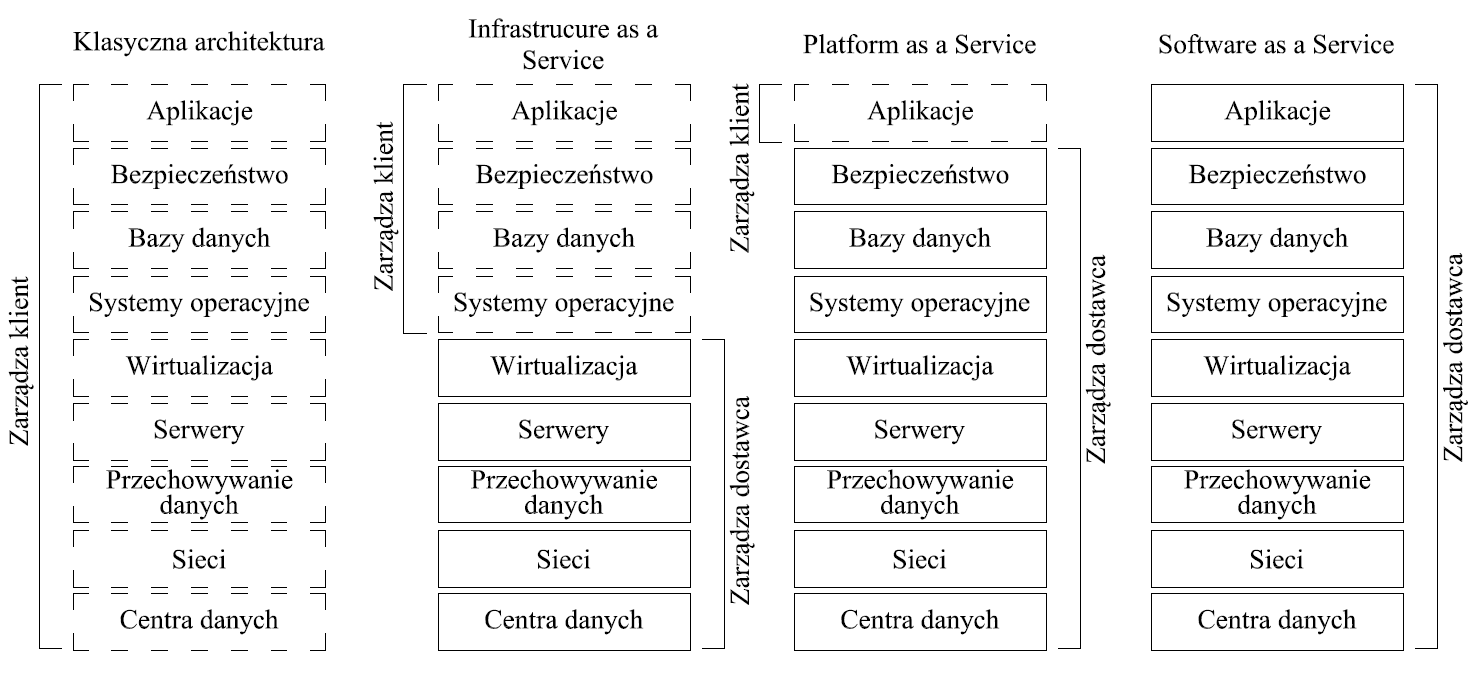
\includegraphics[width=\textwidth, keepaspectratio]{../obrazy/fig:cloudarch.png}
\caption{Stopień ingerencji w oferowane zasoby jest największy w przypadku platformy IaaS, podczas gdy rozwiązania SaaS pozwala użytkownikowi na minimalną inwestycję czasową w zarządzanie infrastrukturą \label{fig:cloudarch}}
\end{figure}

Należy jednak mieć na uwadze, że rozgraniczenie pomiędzy modelem \textit{IaaS} i \textit{PaaS} nie jest aż tak wyraźne jak w przypadku modelu \textit{SaaS}. W niektórych publikacjach \citep{armburst2010} są one traktowane jako grupa rozwiązań, które podzielają więcej podobieństw niż różnic.

\noindent
Modele implementacji:
\begin{itemize}
\item Prywatna chmura (ang. \textit{Private Cloud}) -- infrastruktura zostaje udostępniona na wyłączność dla pojedynczego podmiotu lub organizacji. Może być posiadana i zarządzana przez tę organizację, podmiot trzeci lub dowolną ich kombinację. Może istnieć na terenie dostawcy usług lub poza nim,
\item Zbiorowa chmura (ang. \textit{Community cloud}) -- infrastruktura udostępniona zostaje na wyłączność dla pewnej zbiorowości podmiotów, która mają wspólne cele. Może być posiadana i zarządzana przez jedną lub wiecej z organizacji należących do owej zbiorowości, podmiotu trzeciego lub dowolnej ich kombinacji. Może istnieć na terenie dostawcy usług lub poza nim,
\item Publiczna chmura (ang. \textit{Public cloud}) -- infrastruktura udostępniona dla wszystkich użytkowników. Może być posiadana i zarządzana przez przedsiebiorstwo prywatne lub publiczne, placówkę akademicką lub dowolną ich kombinację. Musi istnieć na terenie dostawcy usług,
\item Hybrydowa chmura (ang. \textit{Hybrid cloud}) -- infrastruktura jest połączeniem dowolnych dwóch lub więcej infrastruktur chmurowych, które pozostają odrębnymi bytami, lecz są związane rozwiązaniami technologicznymi. W przypadku połączenia prywatnej i publicznej chmury pozwala to na utrzymywanie dedykowanej infrastruktury, stanowiącej rdzeń systemu informatycznego przedsiębiorstwa, która w razie wyjątkowego obciążenia systemu lub awarii może zostać wspomagana zasobami pochodzącymi z chmury publicznej, por. \citet{antonopoulos2010}.
\end{itemize}

Ponieważ wiele prywatnych centrów danych korzysta z terminu ,,przetwarzania w chmurze'' w celu opisania swojego modelu biznesowego i przejaskrawienia potencjalnych korzyści, \citet{armburst2010} silnie podkreślają różnicę pomiędzy stosowanymi przez takich dostawców rozwiązaniami, a infrastrukturą posiadającą wszystkie wskazane cechy. Uargumentowane jest to faktem, że ekonomia skali i możliwość błyskawicznego dostosowywania się do zmian w popycie jest w przypadku tego przedsięwzięcia kluczowym czynnikiem, fundamentalnym dla jego opłacalności. Małej i średniej wielkości centra danych (nie posiadające setek tysięcy-milionów serwerów) nie mogą oferować swoim klientom atrakcyjniejszych cen, ponieważ czerpią tylko z podzbioru wymienionych wcześniej możliwości. Ponadto, jak twierdzi \defcitealias{mustafa2015}{Mustafa (2015)}\citetalias{mustafa2015}, paradygmat \textit{cloud computingu} jest w swojej naturze skierowany na potrzeby rynku, podczas gdy klasyczna architektura jest systemocentryczna i nie daje dostawcy bodźców do traktowania wszystkich zgłoszeń z równą wagą. Z wymienionych powodów prywatny model chmury często nie jest przywoływany w debatach nad tego typu rozwiązaniami.

Na tym etapie warto również przywołać pokrewne technologie, takie jak \textit{grid computing} oraz \textit{utility computing}, por. \citet{zhang2010}. \textit{Grid computing}, zwany również przetwarzaniem sieciowym jest paradygmatem rozproszonego przetwarzania danych, który koordynuje zasoby znajdujące się w jednej sieci, by osiągnąć jeden ustalony cel w przetwarzaniu. To rozwiązanie ma swoje korzenie w środowisku naukowym, gdzie wykonywane obliczenia potrzebowały dużej ilości zasobów. Różnica pomiędzy nim a przetwarzaniem w chmurze polega na stopniu wykorzystywania technologii wirtualizacji na wielu poziomach (sprzętowym i aplikacyjnym). Druga z wymienionych technologii, \textit{utility computing}, reprezentuje model dostarczania zasobów na żądanie i fakturowaniu klientów na podstawie ich wykorzystania zamiast stałej stawki. Przetwarzanie w chmurze może być rozpatrywane jako pewnego rodzaju realizacja \textit{utility computingu}. Adaptuje ona schemat ustalania stawek ze względów czysto ekonomicznych.

\subsubsection{Wirtualizacja i zarządzanie zasobami}

\noindent
U podstaw przedstawianej infrastruktury leżą dwie technologie: wirtualizacja oraz zarządzanie zasobami \citep{mustafa2015}. Techniki wirtualizacyjne wykorzystywane są w celu zapewnienia elastycznego i dynamicznego przydzielania mocy obliczeniowej, podczas gdy proces zarządzanie zasobami odpowiada za ich dostarczanie i nadzór nad nimi. Dzieje się to poprzez dzielenie jednej fizycznej maszyny na wiele logicznych systemów operacyjnych z wykorzystaniem hipernadzorcy (ang. \textit{hypervisor}), który emuluje leżący u podstaw model sprzętowy i odpowiada za inicjalizację i nadzorowanie pracy wielu systemów operacyjnych. Rysunek \ref{fig:vm}. przedstawia działanie takiego typu architektury i porównuje go do tradycyjnego podejścia. Wirtualizowany serwer powszechnie nazywany jest maszyną wirtualną (ang. \textit{Virtual Machine, VM}). Cykl życia maszyny wirtualnej obejmuje sześć faz: tworzenie, zawieszenie, wznowienie, zapisanie, migrację oraz niszczenie.

Wirtualizacja po raz pierwszy została wykorzystana na wielką skalę przez IBM w latach 1960 przy systemach klas komputerów określanych jako komputery głównego szeregu (ang. \textit{mainframe systems}). Środowiska wirtualne i systemy operacyjne używane na tych komputerach pozwalały na uruchamianie wielu aplikacji i procesów dla wielu użytkowników jednocześnie i utrzymanie wysokiego poziomu automatyzacji przydzielania zadań. Robert P. Goldberg w 1974 roku opisał potrzebę wykorzystywania maszyn wirtualnych w następujący sposób: ,,Systemy maszyn wirtualnych były oryginalnie zbudowane by naprawić pewne wady architektur trzeciej generacji i wieloprogramowych systemów operacyjnych (ang. \textit{multiprogramming operating systems}, takich jak OS/360'' \citep{goldberg1974}. W latach 1980 i 1990 dominującym podejściem do przetwarzania danych były systemy rozproszeone, aplikacje klient-serwer oraz tanie serwery x86. Osiagnięcia technologiczne ostatnich lat doprowadziły jednak do znacznego wzrostu wydajności stosowania tego typu rozwiązań i wykorzystania wielordzeniowych procesorów na szeroką skalę. Opracowane niedawno, popularne architektury sprzętowe, takie jak rodzina architektur procesorów Intel X86 czy AMD-V silnie czerpią z tego modelu (przykładem mogą również być takie implementacje jak VMware, Xen czy KVM, por. \citet{shroff2010}). Powrót do tego podejścia argumentowany jest także oszczędnością energii \citep{ward2013}, znacznie większą stabilnością tak zaprojektowanego systemu, a w przypadku przedsiębiorstw oferujących usługi przetwarzania w chmurze również możliwością dostosowywania się do błyskawicznie zmieniających się potrzeb konsumentów. Przykładowo w przypadku awarii jednej z maszyn, wszystkie wykonywane przez nią zadania automatycznie zostają migrowane na jedną lub wiele pozostałych jednostek. Ponadto, dostawcy muszą mieć pewność, że są wystarczająco elastyczni, by w czasie rzeczywistym zaspokajać popyt na różne rodzaje jednostek, izolując jednocześnie w wymaganym stopniu użytkowników od fizycznej infrastruktury. To podejście do zarządzania zasobami, ich stałe monitorowanie i możliwość automatycznego reagowania na awaryjne sytuacje muszą być zapewnione w przypadku środowiska \textit{cloud computingowego} i są jego inherentną częścią.

\begin{figure}[h]
  \centering
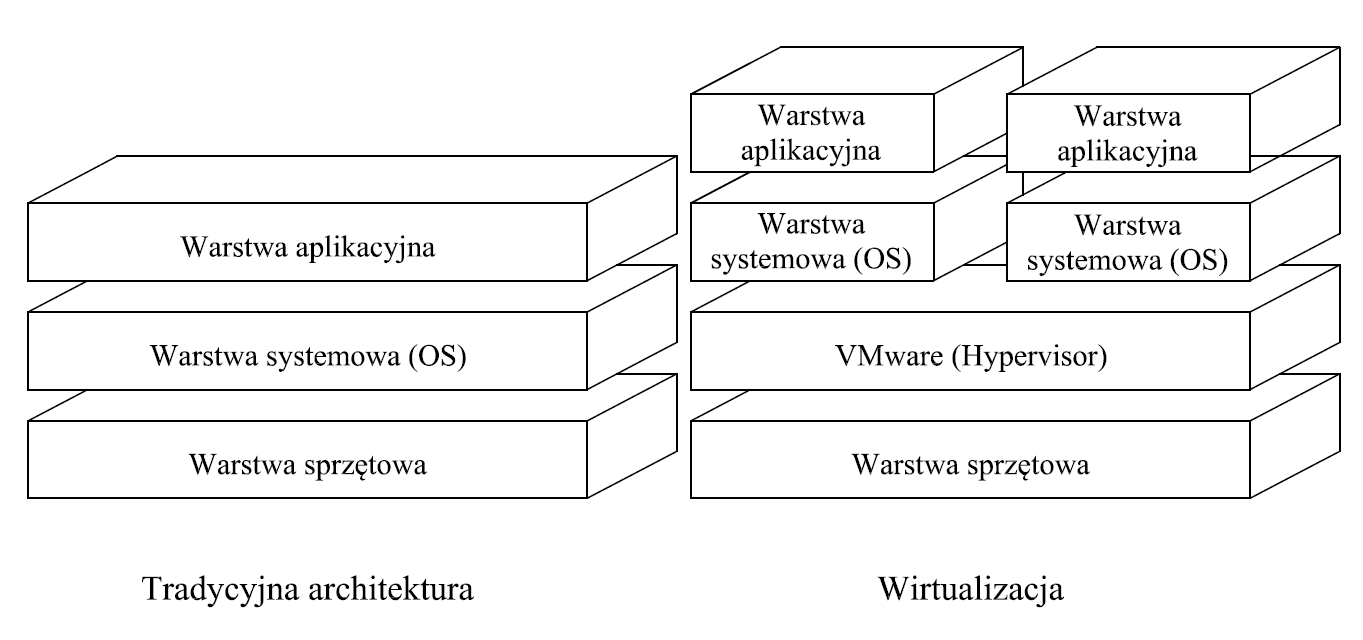
\includegraphics[scale=0.8]{../obrazy/fig:vm.png}
\caption{Wirtualizacja pozwala na uruchomienie licznych maszyn wirtualnych na jednej maszynie fizycznej z wykorzystaniem hipernadzorcy (w tym wypadku \textit{VMware}) \label{fig:vm}}
\end{figure}

Technologia wirtualizacji musi jednak zmierzyć się z pewnymi wyzwaniami. Architektura x86 nie była pierwotnie tworzona jako platforma dedykowana tym rozwiązaniom. Mechanizmy, które pozwalają na tworzenie maszyn wirtualnych na tego typu architekturze wymagają zmodyfikowanego systemu operacyjnego lub używają dodatkowego zestawu instrukcji, dostarczonego przez nowoczesne procesory. Z tego powodu wykorzystywanie wirtualizacji wiąże się z pewnym spadkiem wydajności. Choć według \citet{menon2005} został on w ostatnich latach zminimalizowany, wirtualne maszyny wciąż dostarczają tylko ułamek wydajności równoważnej fizycznej maszyny. Niektóre rodzaje hipernadzorców pozwalają na dostarczenie niemal natywnej wydajności procesora, jednak sedno problemu leży w wydajności procesów wejścia/wyjścia (ang. \textit{input/output (I/O)}), którego spowolnienie może osiągać nawet 88\% w porównaniu do maszyny fizycznej. Ponadto, należy skupić się także na minimalizowaniu strat w przypadku uruchamianie wielu maszyn wirtualnych na jednym rdzeniu procesora. Ponieważ w danym momencie na jednym procesorze może być aktywna tylko jedna maszyna wirtualna, pozostałe z nich pozostają bezczynne i nie mogą odpowiadać na aktywność \textit{I/O}.

\subsubsection{Aspekty ekonomiczne}

\noindent
Przetwarzanie w chmurze stało się jedną z najszybciej rozwijających się gałęzi technologii informacyjnych. W 2009 r. sprzedaż w usługach chmurowych osiągnęła 56 miliardów dolarów \citep{smith2009}, podczas gdy Merryl Lynch przewidywał wzrost wartości rynku do 160 miliardów w 2011. Raport Gartner z 2016 roku \citep{anderson2016} wskazuje, że rynek platform BPaaS, SaaS, Paas oraz Iaas osiągnął w sumie wartość 734 miliardów dolarów, przy czym kolejne 111 miliardów zostanie w niego zainwestowana do 2020 r. Ponieważ uważa się, że technologia ta ma wszelkie argumenty, by fundamentalnie i na stałe zmienić sposób zarządzania zasobami informatycznymi przedsiębiorstwa, dyrektorzy i menedżerowie IT powinni nieustannie śledzić rozwój tej innowacji i dostosowywać do niej swoje długofalowe strategie.

Sukces \textit{cloud computingu} ściśle związany jest z korzyściami ekonomicznymi, które za sobą niesie. Rozwiązanie to pozwala na obniżenie kosztów obsługi, szybszą implementację i większą elastyczność w wykorzystywaniu różnych zestawów narzędzi. Wykorzystanie modeli \textit{pay-as-you-go} skutkuje także minimalizowaniem ryzyka nadmiernego gromadzenia zasobów (ang. \textit{overprovisioning}), jak i ich niewystarczającej ilości (ang. \textit{underprovisioning}). Według \citet{armburst2010} średnie wykorzystanie serwerów w centrach danych wynosi od 5\% do 20\%, co jest spójne z obliczeniami, według których największe obciążenie serwerów przekracza nawet dziesięciokrotnie średnią.  W tym modelu dodatkowe maszyny mogą zostać usunięte lub dodane w ciągu kilku minut (w przeciwieństwie do tygodni-miesięcy w przypadku klasycznego modelu). Efektem tego jest zbilansowana proporcja zapotrzebowania na sprzęt i faktycznego stanu posiadania, co minimalizuje koszty i pozwala uniknąć przeciążania serwerów (zjawisko \textit{overprovisioningu} i \textit{underprovisioningu} zostało zilustrowane na Rysunku \ref{fig:overp}.). Największe korzyści z tego rozwiązania mogą uzyskać te przedsiebiorstwa, które z wykorzystaniem analiz ekonometrycznych potrafią przewidzieć zapotrzebowanie na swoje usługi (tym bardziej jeśli zapotrzebowanie dynamicznie zmienia się na przykład w zależności od pory dnia lub online-owych kampanii reklamowych, jak ma to miejsce w przypadku e-commerce). Ponadto, ta cecha \textit{cloud computingu} ma silny wpływ na jego popularność wśród małych i średnich przedsiębiorstw, które są we wczesnym etapie rozwoju. Promuje ona innowacyjne rozwiązania i pozwala na łatwe znalezienie zasobów koniecznych do ich realizacji. Dlatego też nawet jeśli nabywanie serwerów w modelu \textit{pay-as-you-go} okazuje się droższe niż metoda tradycyjna, może to być atrakcyjniejszą alternatywą ze względu na możliwość szybkiego zwolnienia maszyn bez dodatkowych kosztów.

\begin{figure}[h]
  \centering
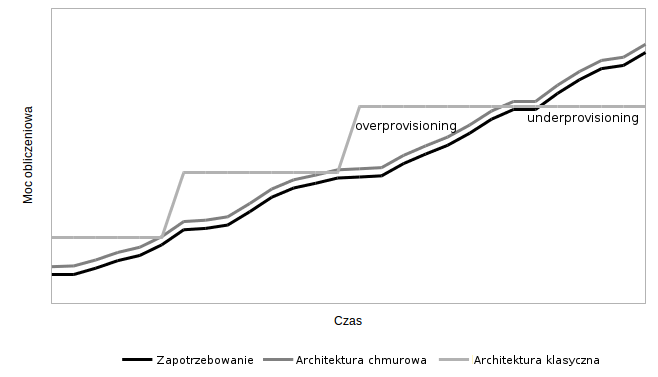
\includegraphics[scale=0.8]{../obrazy/fig:overp.png}
\caption{Tradycyjna architektura wymusza rzadkie zmiany, które skutkują częstym nadmiarem zasobów obliczeniowych. Może on być nawet pogłębiony przez nieoczekiwany spadek zapotrzebowania tuż po zakupieniu dodatkowej mocy obliczeniowej, co generuje dodatkowe koszty. \label{fig:overp}}
\end{figure}

Korzystając z gotowych rozwiązań oferowanych przez dostawców usług \textit{cloud computingowych} klienci mogą również liczyć na zdecydowanie wyższy poziom bezpieczeństwa niż dotychczas, ponieważ ich dane chronione są przez jedno, wysoce wyspecjalizowane w tym zakresie przedsiębiorstwo.

Tego rodzaju model jest także bardzo opłacalny dla dostawców, ponieważ sposób zarządzania tego rodzaju homogenicznym systemem może być optymalizowany. Według \citet{baun2011} konstruowanie wielkoskalowych rozwiązań chmurowych w tanich lokalizacjach pozwala na obniżenie kosztów elektryczności, połączenia sieciowego, operacji, oprogramowania i sprzętu nawet siedmiokrotnie.

Pojawienie się przetwarzania w chmurze miało stymulujący wpływ na gospodarkę, ale także stawia przed sobą wiele nowych wyzwań. W związku z tym, regulatorzy mają również istotną rolę do odegrania w wielu obszarach:
\begin{itemize}
\item bodźce do używania technologii chmurowych -- rządy muszą odegrać rolę w zachęcaniu wykorzystania \textit{cloud computingu} na przykład poprzez usuwanie zbędnych barier prawnych i regylacyjnych, ale również przez bycie wiodącym ich użytkownikiem i zachęcanie do partnerstw publiczno-prywatnych,
\item standardy -- jednym z wielu wyzwań stojących przed rozwojem chmury jest brak odpowiednich standardów w niektórych obszarach, jak również niedostateczne przyjęcie istniejących standardów. Rządy powinny zachęcać i wspierać rozwój otwartych standardów dla wsparcia biznesu, także poprzez współpracę z różnym instytutami normalizacyjnymi,
\item pomiary -- ilość dostępnych publicznie danych o tego typu przedsięwzięciach jest wciąż niewielka. Regulatorzy, w konsultacji z udziałowcami, powinni odegrać istotną rolę w identyfikowaniu stosownych kryteriów pomiaru wyników i oceny stanu tej gałęzi rynku.
\item kraje rozwijające się -- \textit{cloud computing} daje szansę korzystania ze swoich korzyści przy niskich kosztach dla organizacji i konsumentów pochodzących z krajów rozwijających się. Należy zapewnić odpowiednią infrastrukturę sieciową oraz zachęcać do adaptacji i wykorzystania nowych technologii w owych krajach tak, by mogły one doświadczyć wzrostu ekonomicznego, poprawić zdolności edukacyjne, ale również by umożliwić wolny przepływ informacji dla rozwoju społeczeństwa,
\item konkurencja i handel -- ustawodawcy muszą zadbać o to, by nie dopuścić do niekonkurencyjnych praktyk wynikających z dominacji rynkowej kilku niewielkich przedsiębiorstw. Jest to niezwykle istotne, ponieważ (przywołując również teorię \textit{cloud computingu} jako medium) gałęzie rynku, gdzie kluczowym czynnikiem jest ekonomia skali są szczególnie narażone na tego typu sytuację,
\item podatki -- wraz z migracją wielu centrów danych do chmury, należy rozważyć potencjalny wpływ na rozliczenia podatkowe związane z dostarczaniem tych usług. Szczególnie ważna jest to w przypadku przedsiębiorstw, które dotychczas miały niewielkie doświadczenie w transgranicznych transakcjach i rachunkowości,
\item bezpieczeństwo i zarządzanie ryzykiem -- należy wprowadzić regulacje, które pozwolą trafnie zdefiniować stojące przed \textit{cloud computingiem} wyzwania związane z bezpieczeństwem infrastruktury, w szczególności konieczne jest przeprowadzenie oceny ryzyka, zarządzanie bezpieczeństwem i w efekcie jego usprawnienie,
\item prywatność -- regulatorzy powinni zaadresować pojawiające się pytania dotyczące prywatności przechowywanych danych, takich jak: ,,prawa którego państwa stosuje się do danych przechowywanych w chmurze?'', ,,kto ma dostęp do przechowywanych danych?'', ,,w jakich sytuacjach dane mogą zostać udostępnione jednostkom rządowym?''.
\end{itemize}

\subsubsection{Wiodący dostawcy usług \textit{cloud computingowych}}

\noindent
Według najnowszego raportu ,,Magic Quadrant'' firmy Gartner \citep{leong2017}, liderem rynku pozostaje, niezmiennie od 2006 roku, Amazon Web Services, na kolejnych pozycjach plasują się Microsoft, IBM oraz Google (wyniki rankingu przedstawione zostały na Rysunku \ref{fig:mquad}.). Według \citet{forbes2017}, Amazon posiada 31\% udziału w rynku, Microsoft 11\%, podczas gdy IBM i Google odpowiednio 7\% i 5\%. Jednak, pomimo statusu lidera, Amazon musi czynić intensywne wysiłki by zachować swoją pozycję, ponieważ inni wielcy gracze rozwijają się w imponującym tempie, zdobywając coraz większy udział w rynku infrastruktury chmurowej. Microsoft w czwartym kwartale 2015 powiększył swoje obroty o 124\%, podczas gdy w drugim kwartale 2016 roku to Google odnotował największe tempo wzrostu (162\%). Należy jednocześnie zwrócić uwagę na fakt, że czterech największych graczy stopniowo zwiększa swój udział w rynku (z 51\% w czwartym kwartale 2015 do 54\% w drugim kwartale 2016), por. \citet{forbes2017}.

\begin{figure}[h]
  \centering
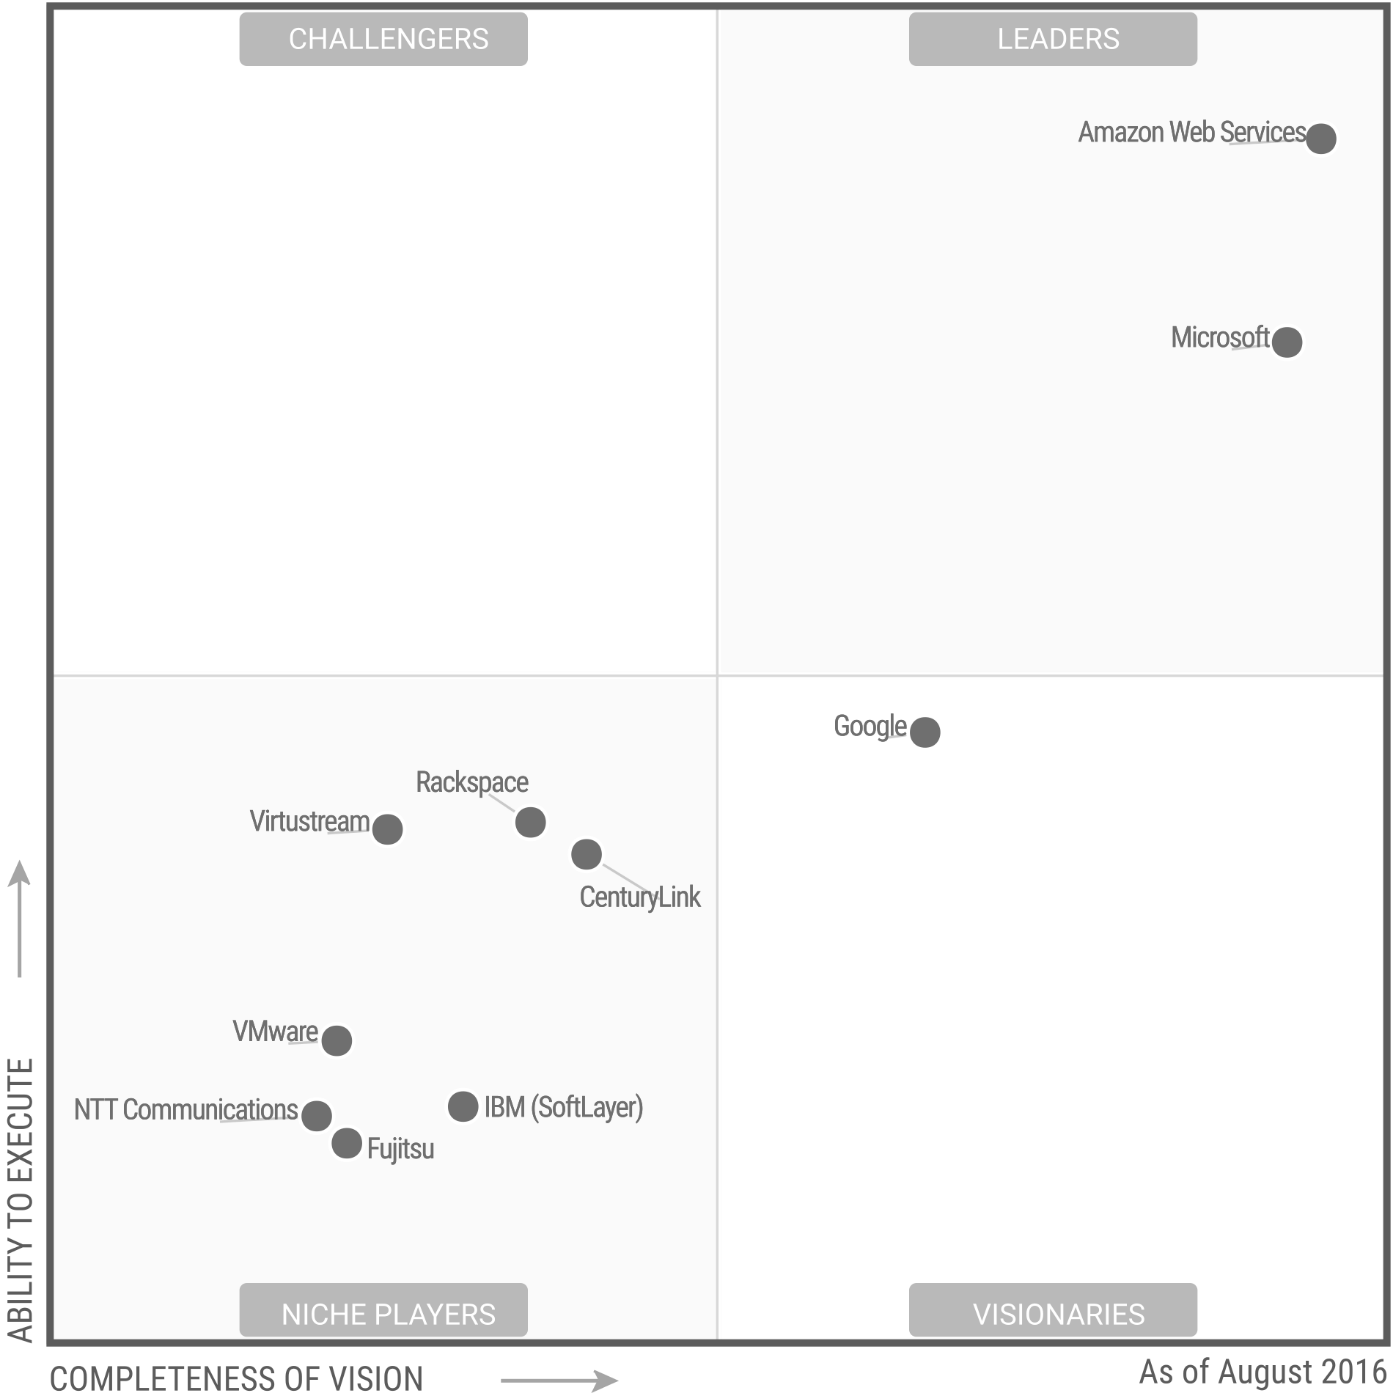
\includegraphics[scale=0.8]{../obrazy/fig:mquad.png}
\caption{\textit{Magic Quadrant} dla przedsiębiorstw oferujących usługi \textit{cloud computingowe} potwierdza status lidera AWS. Należy jednak rozpatrywać Microsoft oraz Google jako równorzędnych konkuretnów. \label{fig:mquad}}
\end{figure}

Amazon, pierwszy dostawca usług przetwarzania w chmurze, przechodził stopniową transformację od portalu oferującego książki do online'owego potentata, wykorzystując jednocześnie wysoce innowacyjne rozwiązania do osiągnięcia tego celu. Ta otwartość na innowacje była niejako wymuszona stopniem skomplikowania oferowanego serwisu. Wyświetlenie jednej strony zawierającej informacje o przedmiocie, rekomendacje oraz oceny wymagało licznych, skomplikowanych aplikacji. Ponadto, detaliczny charakter sprzedaży wymagał ciągłego monitorowania zapotrzebowania na zasoby obliczeniowe, ale również obserwowania popytu i wsparcia  procesów operacyjnych systemami informatycznymi (zarówno swoich, jak i partnerów biznesowych). Amazon wykorzystywał technologię wirtualizacji podobnie, jak wiele innych przedsiębiorstw obecnie, by automatycznie i dynamicznie przydzielać zasoby do aplikacji, które tego potrzebowały w danej chwili. Wysoki stopień automatyzacji, który osiągneli w tym zakresie pozwolił im na uruchomienie ich dwóch największych serwisów -  Amazon EC2 (Elastic Compute Cloud) oraz Amazon S3 (Simple Storage System). Amazon EC2 pozwala użytkownikom chmury uruchamiać serwery i zarządzać nimi w jednym z wielu umiejscowionych na różnych kontynentach centrów danych, podczas gdy Amazon S3 jest usługą służącą do przechowywania danych w chmurze. Usługi te miały początkowo zostać udostępnione wewnętrznie i dla partnerów biznesowych, jednak w ramach eksperymentu otwarto je również dla całego świata, gdzie spotkały się z ogromną popularnością, por. \citet{shroff2010}. Ostatecznie doprowadziło do decyzji o uruchomieniu biznesu \textit{cloud computingowego} w 2006 roku. Od tego czasu AWS znacznie rozszerzyło gamę oferowanych usług i dostarcza swoje usługi z wykorzystaniem centrów danych znajdujących się w Ameryce Północnej, Europie, Azji oraz Ameryce Południowej. Do ich silnych stron zaliczana jest duża liczba klientów, najszerszy wachlarz oferowanych usług oraz największe możliwości obliczeniowe, co doprowadziło do ich partnerstwa technologicznego z licznymi przedsiębiorstwami, które dostosowały swoje produkty do uruchamiania na platformie AWS. Z drugiej strony, wymaga to od początkującego użytkownika dużego nakładu czasu, by zaznajomić się z modelem działania i oferowanymi usługami tak, by mógł dostosować je do swoich potrzeb technologicznych.

Microsoft także coraz bardziej skupia się na dostarczaniu swoich możliwości technologicznych z wykorzystaniem usług chmurowych. Platforma przez nich Azure, pozwala na wynajęcie maszyn wirtualnych (z wykorzystaniem oprogramowania Hyper-V), przechowywanie obiektów w chmurze, jak również wiele innych możliwości IaaS oraz PaaS. Ponadto, Azure Marketplace oferuje oprogramowanie i usługi dostarczane przez inne podmioty. Co więcej, Microsoft błyskawicznie wprowadza nowe usługi i funkcjonalności, nakreślając wizję połączonych modeli IaaS oraz PaaS, które współdziałać będą z istniejącą infrastrukturą \textit{on-premises}.  Centra danych Microsoft (określane mianem ,,regionów'') znajdują się nie tylko w Ameryce Północnej i Południowej, Europie i Azji, ale także w Australii. Wartym odnotowania jest również fakt otwarcia się na technologie open source - gama tego typu rozwiązań wspieranych przez Azure wciąż się poszerza, ze szczególnym uwzględnieniem systemów operacyjnych Linux. Microsoft na pewno będzie również korzystał z istniejących kontaktów biznesowych oraz silnej marki, by promować swój produkt i osiągnąć jeszcze większy udział w rynku technologii chmurowych. Choć Azure daleko do stopnia rozwoju i dojrzałości prezentowanego przez AWS, wiele organizacji określa go jako wystarczająco rozbudowany, by móc w niego inwestować.

IBM, jeden z najstarszych koncernów informatycznych, również oferuje usługi \textit{cloud computingowe}. W celu przyspieszenia ekspansji na rynku, w 2013 roku IBM kupiło SoftLayer, niezależnego dostawcę usług chmurowych, by w efekcie ukształtować IBM Cloud Services Division. Przez kolejne lata następowała stopniowa migracja klientów z IBM SmartCloud Enterprise do SoftLayer. Obecnie oferują zarówno wirtualizowane serwery, jak i klasyczne dedykowane maszyny. Ponadto, istnieje także możliwość przechowywania obiektów poprzez zintegrowany CDN (ang. \textit{Content Delivery Network}. Softlayer oferuje swoje usługi z wykorzystaniem centrów danych znajdujących się w Ameryce Północnej, Europie oraz Azji. Do zalet IBM Softlayer, podobnie jak w przypadku, Microsoft, można zaliczyć silną markę oraz liczne kontakty z klientami na całym świecie, co z pewnością pozwoli na rozwój w segmencie przedsiębiorstw. Należy jednak zaznaczyć, że historycznie Softlayer był głównie skupiony na klasycznym modelu dostarczania mocy obliczeniowej i nie rozróżnia na swoim portalu serwisów chmurowych i niechmurowych, brak jest także wielu możliwości technologicznych charakterystycznych dla przetwarzania w chmurze, oferowanych przez liderów rynku.

Google operuje na rynku PaaS pod 2008 roku (oferując swój App Engine), jednakże w modelu IaaS aktywni są dopiero od udostępnienia światu Google Compute Engine w 2013 roku. Obecnie w swojej ofercie łączą zarówno wymienione usługi, jak również wachlarz dodatkowych możliwości, takich jak możliwość przechowywania danych i Container Engine - usługę pozwalającą na konteneryzację, to znaczy uruchomienie aplikacji w wydzielonym konetenerze, ale bez konieczności emulowania warstwy sprzętowej i systemu operacyjnego. Centra danych Google znajdują się w Ameryce Północnej, Europie i Azji. Przez wiele lat prowadzenia własnego biznesu internetowego, Google nabyło szeroką ekspertyzę w projektowaniu tego typu rozwiązań. Niewątpliwą zaletą korzystania z ich serwisu jest możliwość korzystania z ich osiągnięć technologicznych w zakresie wirtualizacji, wykorzystania kontenerów czy też narzędzi do zarządzania klastrami jak Kubernetes. Należy wszakże zaznaczyć, że zakres usług przez nich oferowany nie jest jeszcze tak szeroki jak w przypadku liderów rynku. Według \citet{leong2017}, pomimo szybkiego tempa wzrostu, Google wciąż nie rozwija się dostatecznie dynamicznie, by móc osiągnąć status lidera w tej gałęzi rynku informatycznego.

%podsumowanko

\clearpage

\begin{thebibliography}{99}
\setlength{\itemsep}{0pt}%
\bibitem[Anderson i Warrilow (2016)]{anderson2016} Anderson, E. i Warrilow, M. (2016). Market Insight: Cloud Shift — The Transition of IT Spending From Traditional Systems to Cloud. Baza danych Gartner
\bibitem[Andrychowicz et al. (2016)]{andrychowicz2016} Andrychowicz, M., Denil, M., Gomez, S., Hoffman, M. W., Pfau, D., Schaul, T. i de Freitas, N. (2016). Learning to learn by gradient descent by gradient descent. In Advances in Neural Information Processing Systems, s. 3981-3989
\bibitem[Antonopoulos i Gilliam (2010)]{antonopoulos2010} Antonopoulos, N. i Gillam, L. (2010). Cloud computing, 1st ed. London: Springer, s. xx - xx
\bibitem[Armburst et al. (2010)]{armburst2010} Armbrust, M., Stoica, I., Zaharia, M., Fox, A., Griffith, R., Joseph, A., Katz, R., Konwinski, A., Lee, G., Patterson, D. i Rabkin, A. (2010). A view of cloud computing. Communications of the ACM, 53(4), s. 50
\bibitem[Baun i Kunze (2011)]{baun2011} Baun, C. i Kunze, M. (2011). Cloud computing. 1st ed. Heidelberg [etc.]: Springer, s. xx -xx
\bibitem[Bengio i Delalleau (2011)]{bengio2011} Bengio, Y. i Delalleau, O. (2011, October). On the expressive power of deep architectures. In International Conference on Algorithmic Learning Theory (s. 18-36). Springer Berlin Heidelberg
\bibitem[Bengio et al. (2007)]{bengio2007a} Bengio, Y., Lamblin, P., Popovici, D. i Larochelle, H. (2007). Greedy layer-wise training of deep networks. Advances in neural information processing systems, 19, 153
\bibitem[Bengio i LeCun (2007)]{bengio2007b} Bengio, Y. i LeCun, Y. (2007). Scaling learning algorithms towards AI. Large-scale kernel machines, 34(5), 1-41
\bibitem[Buyya et al. (2009)]{buyya2009} Buyya, R., Yeo, C., Venugopal, S., Broberg, J. i Brandic, I. (2009). Cloud computing and emerging IT platforms: Vision, hype, and reality for delivering computing as the 5th utility. Future Generation Computer Systems, 25(6), s. 599-616
\bibitem[Carr (2008)]{carr2008} Carr, N. G. (2008). The big switch: Rewiring the world, from Edison to Google. WW Norton and Company, s xx - xx
\bibitem[Calheiros et al. (2010)]{calheiros2010} Calheiros, R., Ranjan, R., Beloglazov, A., De Rose, C. i Buyya, R. (2010). CloudSim: a toolkit for modeling and simulation of cloud computing environments and evaluation of resource provisioning algorithms. Software: Practice and Experience, 41(1), s. 23-50
\bibitem[Chen et al. (2016)]{chen2016} Chen, L. C., Papandreou, G., Kokkinos, I., Murphy, K. i Yuille, A. L. (2016). Deeplab: Semantic image segmentation with deep convolutional nets, atrous convolution, and fully connected crfs. arXiv preprint arXiv:1606.00915
\bibitem[Forbes.com (2017)]{forbes2017} Forbes.com. (2017). Amazon Continues To Gain Share In Cloud Infrastructure Services Market. Dostępne pod adresem: \url{https://www.forbes.com/sites/greatspeculations/2016/08/17/amazon-continues-to-gain-share-in-cloud-infrastructure-services-market/#2277485215b8} (dostęp 11 marca 2017)
\bibitem[Girshick et al. (2014)]{girschick2014} Girshick, R., Donahue, J., Darrell, T. i Malik, J. (2014). Rich feature hierarchies for accurate object detection and semantic segmentation. In Proceedings of the IEEE conference on computer vision and pattern recognition, s. 580-587
\bibitem[Github (2017)]{github2017} GitHub. (2017). Benchmarks for popular convolutional neural network models on CPU and different GPUs, with and without cuDNN. Dostępne pod adresem: \url{https://github.com/jcjohnson/cnn-benchmarks} (dostęp 14 marca 2017)
\bibitem[Goldberg (1974)]{goldberg1974} Goldberg, R. P. (1974). Survey of virtual machine research. IEEE Comput Mag 7(6):34–45
\bibitem[Goodfellow et al. (2016)]{goodfellow2016} Goodfellow, I., Bengio, Y. i Courville, A. (2016). Deep Learning. MIT Press, s. xx - xx
\bibitem[Gysel (2016)]{gysel2016} Gysel P. M. (2016). Ristretto: Hardware-Oriented Approximation of Convolutional Neural Networks. arXiv preprint arXiv:1605.06402
\bibitem[Hacker Noon (2017)]{hackernoon2017} Hacker Noon. (2017). GPUs and Kubernetes for Deep Learning. Dostępne pod adresem: \url{https://hackernoon.com/gpus-kubernetes-for-deep-learning-part-1-3-d8eebe0dd6fe#.jn1xjvpd2} (dostęp 14 marca 2017)
\bibitem[Han et al. (2015)]{han2015} Han, S., Mao, H. i Dally, W. J. (2015). Deep compression: Compressing deep neural networks with pruning, trained quantization and huffman coding. arXiv preprint arXiv:1510.00149
\bibitem[Han et al. (2016)]{han2016} Han, S., Liu, X., Mao, H., Pu, J., Pedram, A., Horowitz, M. A. i Dally, W. J. (2016) EIE: Efficient Inference Engine on Compressed Deep Neural Network. arXiv preprint arXiv:1602.01528, 2016a
\bibitem[Hebb (1949)]{hebb1949} Hebb, D.O. (1949). The Organization of Behavior. New York: Wiley and Sons
\bibitem[Hecht-Nielsen (1988)]{hecht1988} Hecht-Nielsen, R. (1988). Theory of the backpropagation neural network. Neural Networks, 1, s. 445
\bibitem[Hinton (2006)]{hinton2006} Hinton, G. (2006). Reducing the Dimensionality of Data with Neural Networks. Science, 313(5786), s. 504-507
\bibitem[Hinton i Sejnowski (1986)]{hinton1986} Hinton, G. E. i Sejnowski, T. J. (1986). Learning and relearning in Boltzmann Machines. Parallel Distributed Processing, Rumelhart et al, Eds
\bibitem[Hinton et al. (2006)]{hintonetal2006} Hinton, G., Osindero, S. i Teh, Y. (2006). A Fast Learning Algorithm for Deep Belief Nets. Neural Computation, 18(7), s. 1527-1554
\bibitem[Hinton et al. (2012)]{hinton2012} Hinton, G., Deng, L., Yu, D., Dahl, G., Mohamed, A., Jaitly, N., Senior, A., Vanhoucke, V., Nguyen, P., Sainath, T. i Kingsbury, B. (2012). Deep Neural Networks for Acoustic Modeling in Speech Recognition: The Shared Views of Four Research Groups. IEEE Signal Processing Magazine, 29(6), s. 82-97
\bibitem[Jermain et al. (2015)]{jermain2015} Jermain, C. L., Rowlands, G. E., Buhrman, R. A., i Ralph, D. C. (2015). GPU-accelerated micromagnetic simulations using cloud computing. arXiv preprint arXiv:1505.01207
\bibitem[Kleinrock (2005)]{kleinrock2005} Kleinrock, L., A Vision for the Internet. ST Journal for Research, tom 2, nr 1, s. 4–5
\bibitem[Krizhevsky et al. (2012)]{krizhevsky2012} Krizhevsky, A., Sutskever, I. i Hinton, G. (2012). Imagenet classification with deep convolutional neural networks. In Advances in neural information processing systemsk, s. 1097-1105
\bibitem[LeCun, Bengio i Hinton (2015)]{lecun2015} LeCun, Y., Bengio, Y. i Hinton, G. (2015). Deep learning. Nature, 521(7553), s.436-444
\bibitem[Leong et al. (2017)]{leong2017} Leong, L., Petri, G., Gill, B. i Dorosh, M. (2017). Magic Quadrant for Cloud Infrastructure as a Service. Gartner.com. Dostępne pod adresem: \url{https://www.gartner.com/doc/reprints?id=1-2G2O5FC&ct=150519} (dostęp 11 marca 2017)
\bibitem[Litvinenko (2014)]{litvinenko2014} Litvinenko, N. (2014). Using of GPUs for cluster analysis of large data by K-means method arXiv preprint arXiv:1402.3788
\bibitem[McCulloch i Pitts (1943)]{mcculloch1943} McCulloch, W. S. i Pitts, W. (1943). A logical calculus of the ideas immanent in nervous activity. The bulletin of mathematical biophysics, 5(4), s. 115-133
\bibitem[Medium (2017a)]{medium2017a} Medium (2017). TensorFlow 1.0 is here. Let’s do some Deep Learning on the Amazon Cloud! – Sigmoidal. Dostępne pod adresem: \url{https://medium.com/sigmoidal/tensorflow-1-0-is-here-lets-do-some-deep-learning-on-the-amazon-cloud-9234eab31fa5#.vyxzk4bwk} (dostęp 14 marca 2017)
\bibitem[Medium (2017b)]{medium2017b} Medium (2017). Keras with GPU on Amazon EC2 – a step-by-step instruction. Dostępne pod adresem: \url{https://medium.com/@mateuszsieniawski/keras-with-gpu-on-amazon-ec2-a-step-by-step-instruction-4f90364e49ac#.i2rxriv4g} (dostęp 14 marca 2017)
\bibitem[Mell i Grance (2011)]{mell2011} Mell, P. i Grance T. (2011). The NIST definition of cloud computing
\bibitem[Menon et al. (2005)]{menon2005} Menon, A., Santos, J., Turner, Y., Janakiraman, G. i Zwaenepoel, W. (2005). Diagnosing performance overheads in the xen virtual machine environment. Proceedings of the 1st ACM/USENIX international conference on Virtual execution environments - VEE '05
\bibitem[Minsky i Papert (1969)]{minsky1969} Minsky, M. i Papert, S. (1969). Perceptrons
\bibitem[Mnih et al. (2013)]{mnih2013} Mnih, V., Kavukcuoglu, K., Silver, D., Graves, A., Antonoglou, I., Wierstra, D. i Riedmiller, M. (2013). Playing atari with deep reinforcement learning. arXiv preprint arXiv:1312.5602
\bibitem[Mustafa et al. (2015)]{mustafa2015} Mustafa, S., Nazir, B., Hayat, A., Khan, A. i Madani, S. (2015). Resource management in cloud computing: Taxonomy, prospects, and challenges. Computers and Electrical Engineering, 47, s. 186-203
\bibitem[OECD (2014)]{oecd2014} OECD (2014). Cloud Computing: The Concept, Impacts and the Role of Government Policy. OECD Digital Economy Papers, No. 240, OECD Publishing, Paris
\bibitem[Rosenblatt (1957)]{rosenblatt1957} Rosenblatt, F. (1957). The Perceptron--a perceiving and recognizing automaton. Report 85-460-1, Cornell Aeronautical Laboratory
\bibitem[Rumelhart et al. (1986)]{rumelhart1986} Rumelhart, D. E., Hinton, G. E. i Williams, R. J. (1986). Learning representations by back-propagating errors. Nature, 323, 533-536.
\bibitem[Shetty (2016)]{shetty2016} Shetty, S. (2016).  Application of Convolutional Neural Network for Image Classification on Pascal VOC Challenge 2012 dataset. arXiv preprint arXiv:1607.03785
\bibitem[Shroff (2010)]{shroff2010} Shroff, G. (2010). Enterprise cloud computing. 1st ed. Cambridge: Cambridge University Press, s. xx - xx
\bibitem[Smith et al. (2009)]{smith2009} Smith D. M. et al. (2009). Hype Cycle for Cloud Computing (ID: G00168780). Baza danych Gartner
\bibitem[Srivastava et al. (2014)]{srivastava2014} Srivastava, N., Hinton, G. E., Krizhevsky, A., Sutskever, I. i Salakhutdinov, R. (2014). Dropout: a simple way to prevent neural networks from overfitting. Journal of Machine Learning Research, 15(1), s. 1929-1958
\bibitem[Strom (2015)]{strom2015} Strom, N. (2015). Scalable distributed DNN training using commodity GPU cloud computing. INTERSPEECH (tom 7, s. 10)
\bibitem[Szegedy (2014)]{szegedy2014} Szegedy, C. et al. (2014). Going deeper with convolutions. arXiv preprint arXiv:1409.4842
\bibitem[Touretzky i Hinton (1985)]{touretzky1985} Touretzky, D. S. i Hinton, G. E. (1985, August). Symbols among the neurons: Details of a connectionist inference architecture. In IJCAI (tom 85, s. 238-243)
\bibitem[Vanhoucke et al. (2011)]{vanhoucke2011} Vanhoucke, V., Senior, A. i Mao, M. Z. (2011). Improving the speed of neural networks on CPUs. In Proc. Deep Learning and Unsupervised Feature Learning NIPS Workshop (tom 1, s. 4)
\bibitem[Von Melchner et al. (2000)]{vonmelchner2000} Von Melchner, L., Pallas, S. L. i Sur, M. (2000). Visual behaviour mediated by retinal projections directed to the auditory pathway. Nature, 404(6780), 871-876
\bibitem[Ward i Baker (2013)]{ward2013} Ward, J.S. i Barker, A. (2013). A Cloud Computing Survey: Developments and Future Trends in Infrastructure as a Service Computing
\bibitem[Widrow i Hoff (1960)]{widrow1960} Widrow, B. i Hoff, M. E. (1960, August). Adaptive switching circuits. In IRE WESCON convention record (tom 4, nr 1, s. 96-104)
\bibitem[Zhang et al. (2010)]{zhang2010} Zhang, Q., Cheng, L. i Boutaba, R. (2010). Cloud computing: state-of-the-art and research challenges. Journal of Internet Services and Applications, 1(1), s. 7-18

\end{thebibliography}
\clearpage

\listoffigures

\clearpage

\listoftables

\clearpage

\end{document}
